\chapter{Introduction} % Write in your own chapter title
\label{Chapter1}
\lhead{Chapter 1. \emph{Introduction}} % Write in your own chapter title to set the page header

\section{Introduction}

Surveillance cameras has become popular and placed almost everywhere, e.g. train stations, airports, banks, shops, streets. The balance between security and privacy is still an open problem for researchers and is an active subject for political/social debate. It is hard to keep a balance between security and privacy, a person may feel protected when he knows himself and his surroundings are being observed, but at the same time he may feel uncomfortable because he does not know how many cameras are set and from what angle they are pointing at him.

The information that a person probably wants to know most about surveillance cameras is their viewing fields, e.g. where the camera are, whether the person is inside the observed area. For indoor environment, because the space is usually small, people may easily locate and estimate the viewing fields of the cameras. For outdoor environment, it is almost impossible to find surveillance camera systems which support people to visually see the viewing fields in real scene. Fortunately, there is a technology which can be applied for situations like this: MR (Mixed Reality). MR is the encompassing of both Augmented Reality and Augmented Virtuality, merging real world in which we are living and virtual worlds created by computers. MR produces new environments where real and virtual entities can co-exist and interact in realtime \citep{Reference3}.

MR applications are traditionally equipped with HMD (Head Mounted Display) as shown in figure \ref{fig:HMD}. However, HMDs are usually bulky and inconvenient for outdoor applications, where wide-range mobility is crucial. In recent years, mobile devices has become popular, devices like cell phones, PDA (Personal Digital Assistants) can be seen everywhere. Their prices have come down and they could reach the hands of common people even in developing countries like Viet Nam. High-end mobile devices, such as Apple iPhone and Google T-Mobile G1, usually have high specifications. More importantly for outdoor MR applications, they are equipped with built-in cameras, GPS (Global Positioning System), and accelerometer devices. These auxiliary devices usually meet the need of common outdoor MR applications because they provide video and information to help tracking and mapping the position and orientation of the mobile devices \citep{Reference2} \citep{Reference4}.

\begin{figure}[htbp]
	\centering
	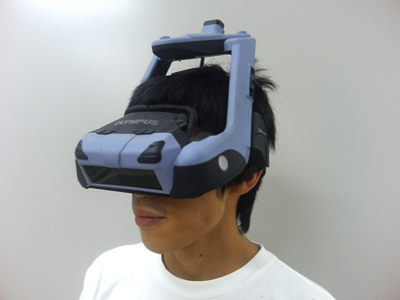
\includegraphics{./Primitives/hmd.jpg}
	\rule{35em}{0.5pt}
	\caption[An HMD]{An HMD}
	\label{fig:HMD}
\end{figure}

However, image processing applications usually need large memory and powerful computing capability. Even current high-end cell phones and PDA may not run MR applications properly without special tweaking. For compute-intensive outdoor MR applications, more powerful UMPC (Ultra-Mobile Portable Computer) devices like the one in figure \ref{fig:VAIO} may be used. UMPC equipped with built-in camera, GPS, and gyrocompass devices has been found practical and are a topic of many researches \citep{Reference2} \citep{Reference4}. Such devices find their high potential use in outdoor MR applications and researches because of their small size, high specifications, and competitive prices.

\begin{figure}[htbp]
	\centering
	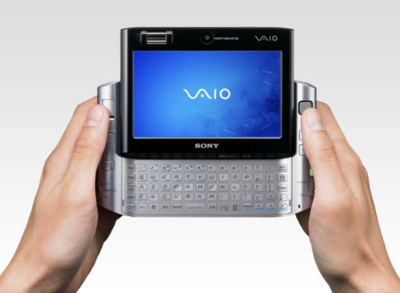
\includegraphics{./Primitives/vaio.png}
	\rule{35em}{0.5pt}
	\caption[SONY VAIO VGN-UX90PS with a camera at the front]{SONY VAIO VGN-UX90PS with a camera at the front (top, center)}
	\label{fig:VAIO}
\end{figure}

\begin{figure}[htbp]
	\centering
	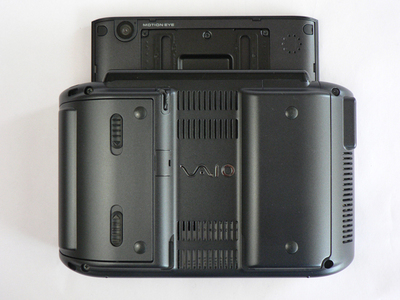
\includegraphics{./Primitives/vaio_back.jpg}
	\rule{35em}{0.5pt}
	\caption[SONY VAIO VGN-UX90PS with a camera at the back]{SONY VAIO VGN-UX90PS with a camera at the back (top, left)}
	\label{fig:VAIOBack}
\end{figure}

In this research, we propose:

\begin{itemize}
	\item Five methods to visualize the viewing fields of surveillance cameras on mobile device screen (chapter \ref{Chapter3}).
	\item A prototype implementation based on server-side PTAM (Parallel Tracking and Mapping) \citep{Reference12} technology (chapter \ref{Chapter4}). The prototype uses a Sony VAIO VGN-UX90PS (appendix \ref{AppendixA}) and provides realtime video. Because the VAIO is still weak to do PTAM processing, we connect it wirelessly to an Apple MacBook Pro, which actually does the heavy work of PTAM. This results in a prototype providing realtime video without any GPS and gyrocompass devices.
\end{itemize}

An experiment to evaluate the visualization methods is described in chapter \ref{Chapter5}.

\section{A Use Case}
\label{AUseCase}

Using the prototype we make in chapter \ref{Chapter4}, when a user wants to see the visualized viewing fields of surrounding surveillance cameras on his own mobile device screen, the typical usage scenario is (see figure \ref{VAIOMacBookPro}):

\begin{enumerate}
	\item The user points the mobile camera in a certain direction.
	\item Through wireless network, the mobile device continuously sends frames captured by the camera of the scene to a more powerful remote computer for processing.
	\item Based on pre-registered data and the frames, the remote computer continuously tracks and maps the position and orientation of the mobile camera, and send them to the mobile device.
	\item Based on pre-registered 3D model of the scene and the position and orientation data, the mobile device correctly renders virtual CG (computer graphics) objects onto the frame to visualize the viewing field of the surrounding surveillance cameras, and renders the resulted image onto its screen. In this research we study five visualization methods. They are described in detail in chapter \ref{Chapter3}.
\end{enumerate}

\begin{figure}[htbp]
	\centering
	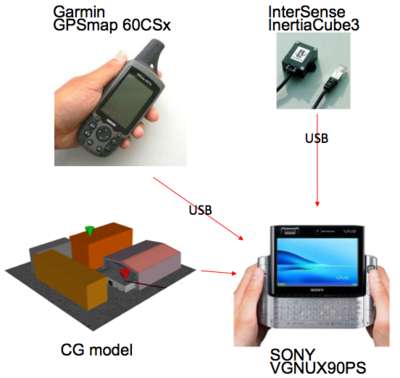
\includegraphics{./Primitives/vaio_macbookpro.png}
	\rule{35em}{0.5pt}
	\caption[Prototype architecture]{Prototype architecture}
	\label{fig:VAIOMacBookPro}
\end{figure}

[FIXME: replace the image]

The system is described in detail in chapter \ref{Chapter4}. It provides realtime video. When the user changes the position or orientation of the mobile camera, the video displayed on the screen will simultaneously change accordingly to the camera movement.

The purpose of the above use case is to give one example of application of visualizing viewing fields of surveillance cameras and to give a rough idea of how the prototype works. There may be other applications. For example, we can build a system which visualizes ``safe paths'' or ``safe areas'' for pupils, as in figure \ref{fig:HomeSchool}. Pupils can use their cell phones to see if their current location is being well observed when they walk to school or go home from school.

\begin{figure}[htbp]
	\centering
	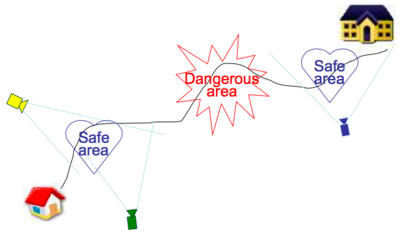
\includegraphics{./Primitives/home_school.png}
	\rule{35em}{0.5pt}
	\caption[Safe path to school]{Safe path to school}
	\label{fig:HomeSchool}
\end{figure}
